\chapter{Introduction}

In this chapter, we first describe sequence tagging tasks and introduce the motivation of this thesis. Then, we summarize our major contributions and describe the structure of the thesis.

\section{Sequence Tagging Task}

\subsection{Part-of-Speech Tagging (POS)}
Part-of-Speech Tagging (POS) is a basic sequence tagging task, which assigns each word with a unique tag that indicates its syntactic role, such as noun, adverb, verb, etc. Figure \ref{fig:pos-ex} illustrates a typical POS task. 

\begin{figure}
  \centering
  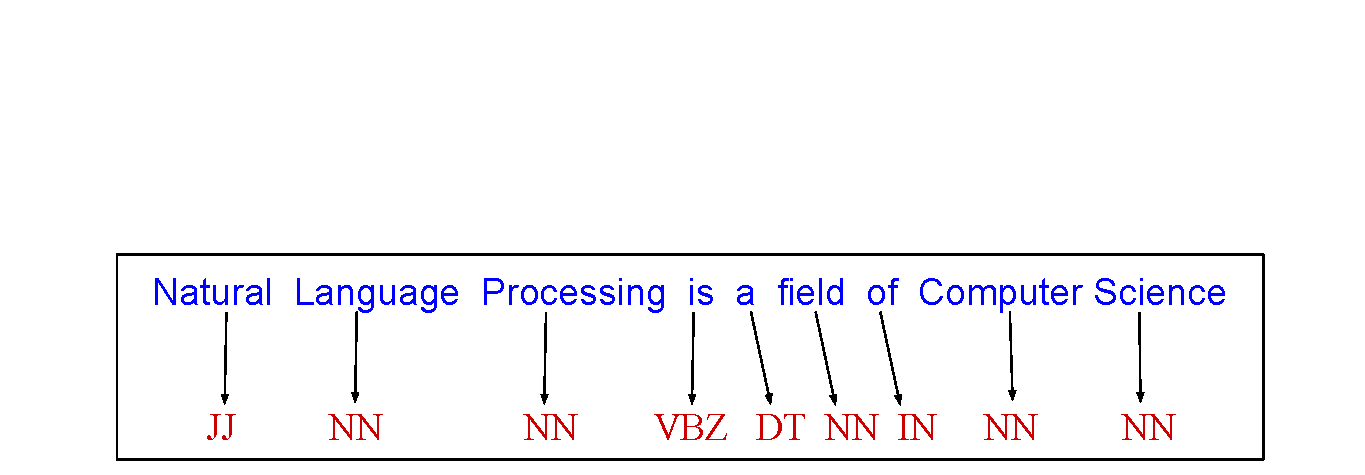
\includegraphics[scale=0.6]{posex.pdf}
 \caption{An example of POS}
  \label{fig:pos-ex}
\end{figure}

Most POS systems are evaluated on the English Penn TreeBank data set (\citeauthor{marcus1993building}, \citeyear{marcus1993building}), which contains 45 part-of-speech tags. The standard split uses section 1-18 of the Treebank for training, section 19-21 for tuning, and section 22-24 for testing (\citeauthor{toutanova2003feature}, \citeyear{toutanova2003feature}). The experimental data are summarized in Table \ref{table:my-dataset}. Many existing models are linear models, such as Maximum entropy Markov models (MEMMs) which obtain 96.46\% per word accuracy (\citeauthor{mccallum2000maximum}, \citeyear{mccallum2000maximum}); and the averaged perception discriminative model which obtains 97.11\% per word accuracy (\citeauthor{collins2002discriminative}, \citeyear{collins2002discriminative}). More recently, neural network models have been proposed to improve the state-of-the-art score. The Bidirectional LSTM network model proposed by \cite{huang2015bidirectional} reaches 97.55\% per word accuracy. \cite{ling2015finding} presents the compositional character-to-word LSTM model which reaches the state-of-the-art performance: 97.78\% per word accuracy. 

\begin{table}[]
\centering
\caption{Number of Words and Labels in Each Training, Validation and Test Section of Different Data Sets}
\label{table:my-dataset}
\begin{tabular}{|c|c|c|c|c|} \hline
      & Training  & Validation  & Test  & labels  \\ \hline
Penn Treebank   &950011 &40068 &56671 &45 \\\hline
CoNLL 2000   &211727 & N/A   &47377 &22   \\\hline
CoNLL 2003   &204567 &51578 &46666 &9     \\\hline
OntoNotes   &1088503 &147724 &152728 &18     \\\hline
\end{tabular}
\end{table}

\subsection{Named Entity Recognition (NER)}

\begin{figure}
  \centering
  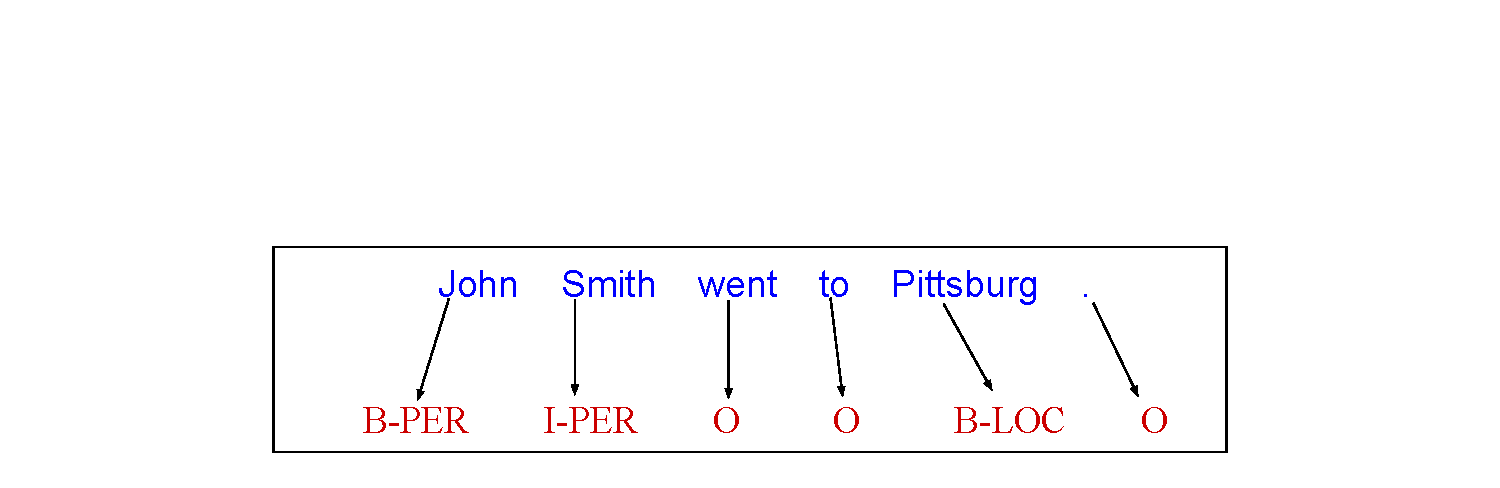
\includegraphics[scale=0.6]{nerex.pdf}
 \caption{An example of NER}
  \label{fig:ner-ex}
\end{figure}

Named Entity Recognition (NER) identifies expressions
that refer to named entities, such as people, places, organizations and others. The main difference between NER and POS is that each named entity label can span multiple words while each part-of-speech tag is only for one word. A popular convention in NER is to use the "IOB" label scheme (Inside, Outside, Beginning): if the word is the beginning of a named entity label, it is marked with B-label; if the word is inside a named entity label but not the first one, it is marked with I-label; if the token is outside the named entity, it is marked with "O". An example of NER is shown in Figure \ref{fig:ner-ex}. There are different numbers of named entity types in different NER tasks. For example, the shared task of CoNLL 2003 (\citeauthor{tjong2003introduction}, \citeyear{tjong2003introduction}) contains 4 types of named entities: locations (LOC), persons (PER), organizations (ORG), and miscellaneous (MISC); and the OntoNotes English data set (\citeauthor{hovy2006ontonotes}, \citeyear{hovy2006ontonotes}) contains 18 types of named entities shown in Table \ref{table:ontonotes-type}. The predefined training, development, and testing split of the data sets are shown in Table ~\ref{table:my-dataset}.

\begin{table}[]
\centering
\caption{Name Entity Types in OntoNotes}
\label{table:ontonotes-type}
\begin{tabular}{|c|c|} \hline
Types  & Named Entities  \\ \hline
PERSON & People, including fictional \\ \hline
NORP & Nationalities or religious or political groups \\\hline
FACILITY & Buildings, airports, highways, bridges, etc. \\ \hline
ORG & Companies, agencies, institutions \\ \hline
GPE & Countries, cities, states \\ \hline
LOC & Non-GPE locations, mountain ranges, bodies of water \\ \hline
PRODUCT & Vehicles, weapons, foods, etc. (Not services) \\ \hline
EVENT & Named hurricanes, battles, wars, sports events \\ \hline
WORK OF ART & Titles of books, songs \\ \hline
LAW & Named documents made into laws \\ \hline
LANGUAGE & Any named language  \\ \hline
DATE & Absolute or relative dates or period \\ \hline
TIME & Times smaller than a day  \\ \hline 
PERCENT & Percentage \\ \hline
MONEY & Monetary values, including unit \\ \hline
QUANTITY & Measurements, as of weight or distance \\ \hline
ORDINAL & First, Second, etc. \\ \hline
CARDINAL & Numerals that do not fall under another type \\ \hline
\end{tabular}
\end{table}

Most NER models are evaluated on CoNLL 2003 data set and are measured by the F1 score, which is the harmonic mean of precision and recall. 

\begin{equation}\label{eqn:softmax}
F_{1} = 2\times \dfrac{\textit{precision} \times \textit{recall}}{\textit{precision} + \textit{recall}}
\end{equation}

Since CoNLL 2003 has a relatively smaller amount of training data, most of the existing models make use of pretrained word embeddings along with the training data. A commonly used pretrained word embedding is GloVe (\citeauthor{pennington2014glove}, \citeyear{pennington2014glove}) which contains 40K words. The best system presented at the NER CoNLL 2003 challenge by \cite{florian2003named} obtains 88.76 F1 score. The model using Bidirectional LSTM by \cite{huang2015bidirectional} reaches 88.83 F1 score. Both of these two models use many external features along with a gazetteer\footnote{Gazetteers are language-specific knowledge resources}. \cite{lample2016neural} proposed two NER models with no external features or a gazetteer: the first one makes structured prediction using Bidirectional LSTM, Character Embeddings (\citeauthor{ling2015finding}, \citeyear{ling2015finding}) and Conditional Random Fields (CRF) (\citeauthor{lafferty2001conditional}, \citeyear{lafferty2001conditional}); and the second one uses a Shift-Reduce framework with Stack-LSTM (\citeauthor{dyer2015transition}, \citeyear{dyer2015transition}). The first model achieves 90.94 F1 score, while the second one performs slightly worse and achieves 90.33 F1 score. 

\subsection{Chunking}

Chunking is also known as shallow parsing which labels segments of a sentence with syntax tags, such as NP, VP, PP, etc.  An example of chunking is shown in Figure \ref{fig:ner-ex} The main difference between chunking and POS is that each chunking tag can span multiple words while each part-of-speech tag is only for one word. The "IOB" label scheme is used in chunking. An example of NER is shown in Figure \ref{fig:chunk-ex}. The best system using SVMs presented at the CoNLL 2000 challenge by \cite{Kudoh:2000:USV:1117601.1117635} obtains 93.48 F1 score. The current state-of-the-art score is 95.23 which is achieved by \cite{shen2005voting}. They use part-of-speech tags as features and a voting classifier for chunking. Recently, \cite{huang2015bidirectional} employs Bidirectional LSTM to solve chunking and achieved 94.46 F1 score with a number of hand-crafted features.
\begin{figure}
  \centering
  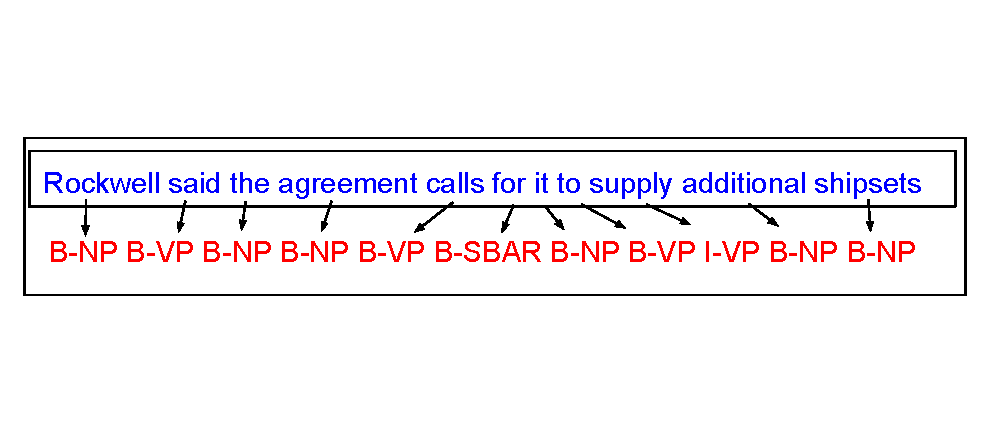
\includegraphics[scale=0.8]{Chunkingex.pdf}
 \caption{An example of Chunking}
  \label{fig:chunk-ex}
\end{figure}

\section{Motivation}
Recurrent Neural Networks (RNNs) have obtained impressive results in many NLP tasks, such as speech recognition (\citeauthor{graves2013speech}, \citeyear{graves2013speech}) and machine translation (\citeauthor{cho2014properties}, \citeyear{cho2014properties}).
Bidirectional Long Short Term Memory (BiLSTM) (\citeauthor{Hochreiter97longshort-term}, \citeyear{Hochreiter97longshort-term}; \citeauthor{graves2005framewise}, \citeyear{graves2005framewise}) is one of the RNN architectures that can maintain long-distance information from the past and future elements in an input sequence. Based on the existing work (POS system by \cite{ling2015finding} and NER system by \cite{lample2016neural}), state-of-the-art results on POS and NER can be obtained by using a BiLSTM network with Character Embeddings and Conditional Random Fields (CRF). Some work has also shown that feedforward neural networks can achieve comparable accuracy to recurrent models in tasks such as POS and Dependency Parsing (\citeauthor{andor2016globally}, \citeyear{andor2016globally}). One approach presented in this thesis is to employ a greedy transition system with a feedforward network to make independent classification decisions on each word. While the state-of-the-art model focuses on the sentence level and computes the score of every possible output sequence during decoding, the greedy system makes decisions on word level and can produce output sequence faster. However, the greedy system is limited when there are strong correlations between output labels. NER is one such task which has grammar constraints on output label sequences. For example, "I-PER" cannot follow "B-LOC" in NER. Next, we want to build a fast neural network model that can capture the dependencies among output tags.

Since the labels in Chunking and NER often span multiple tokens, most neural architectures for chunking and NER predict the boundaries and types of entities together using the "IOB" label scheme. Mention2Vec (\citeauthor{stratos2016mention2vec}, \citeyear{stratos2016mention2vec}) is proposed to address the natural segment-level representation by separating the NER task into boundary detection (I, O, B) and type prediction (PER, LOC, etc.). While Mention2Vec employs two BiLSTMs for each sub-task, we replace the BiLSTM layer for boundary detection with a feedforward network in order to obtain a simpler and faster model. This new model is denoted as Feedforward-Mention2Vec in this thesis.

We use Byte Pair Encoding (BPE) (\citeauthor{gage1994new}, \citeyear{gage1994new}) to deal with rare words in sentences for machine translation (\citeauthor{sennrich2015neural}, \citeyear{sennrich2015neural}), and we propose a new model combining BPE and Mention2Vec for POS, which is denoted as BPE-Mention2Vec in this thesis. We use BPE to segment the input words in the hope of capturing the orthographic evidence of the words without using spelling features (like prefixes and suffixes) or Character Embeddings. After we segment input words, POS becomes an NER-like task. Then, we can use Mention2Vec to solve the rest of the problem. Since boundaries of output tags are known in POS, we only need to use a BiLSTM network for type prediction in \mb.

There is increasing demand for faster sequence tagging systems to decode real time natural language data, such as Twitter, Facebook, Wikipedia, and even the web. Improving decoding speed will benefit many real world sequence tagging applications, but there is very little research into examining the decoding speed and accuracy relationship of different models. In this thesis, we will explore the speed and accuracy trade-off in different neural network models for sequence tagging. We re-implement many different types of feedforward models and BiLSTM models using Tensorflow (\citeauthor{abadi2016tensorflow}, \citeyear{abadi2016tensorflow}) and systematically compare the performance and decoding speed between them on sequence tagging tasks, such as POS and NER.

\section{Contribution}
The three main contributions of this thesis are:

\begin{enumerate}

\item  We implement the state-of-the-art sequence tagging model:BiLSTM with Character Embeddings and CRF, and we apply the fully structured BiLSTM model on all three sequence tagging tasks.

There is little work examining how the configurations of the fully structured BiLSTM model affect the decoding speed, such as whether the model is using Character Embeddings or the model is using CRF. We conduct experiments to compare the performance and decoding time of different configurations. 

\item We build a greedy tagging system with a feedforward neural network: \ffa. 

\ffa{} takes word features in context, spelling features, and previous tag features as input, and uses a feedforward neural network to predict tags word by word. There is little existing work measuring the decoding time using feedforward networks on sequence tagging, so we conduct experiments on sequence tagging and record the performance and decoding speed. To test the robustness of the feedforward networks, we also conduct experiments using a feedforward network with only word features, which also serves as the baseline. We compare the  feedforward model with the fully structured BiLSTM model and provide analysis on the results. 


\item Last but not least, we introduce two new neural architectures based on Mention2Vec: Feedforward-Mention2Vec for chunking and NER, and BPE-Mention2Vec for POS. 

Originally, Mention2Vec was designed for NER and used BiLSTMs to detect named entity boundaries and predict corresponding types separately. We propose Feedforward-Mention2Vec for Chunking and NER, in which we use a feedforward network with CRF to predict named entity boundaries instead of using a BiLSTM.  We denote this new model as \ma. We also adapt Mention2Vec for POS by combining Byte Pair Encoding (BPE) with BiLSTM in the model. BPE is used to segment the input words in our model, and it converts POS into a NER-like task. We denote this new model for POS as \mb. In BPE-Mention2Vec, we use a feedforward network to compute the hidden embeddings of the input segmented words. Since the boundaries of subword units are known, \mb{} does not need to predict the boundaries. It takes the hidden embeddings, tag boundaries, and a BiLSTM network to predict the actual POS tags. We benchmark these two multitask models against the state-of-the-art BiLSTM model on POS and NER. Since different NER tasks have different numbers of named entity types, the decoding time of a fully structured BiLSTM model grows quadratically in the number of types. In Mention2Vec and Feedforward-Mention2Vec, we only apply CRF on boundary labels ('I', 'O', 'B'), so the decoding time grows linearly in the number of types. To show the time difference on different NER tasks, we conduct the NER experiments on CoNLL 2003 which contains 4 different named entity types and OntoNotes which contains 18 different named entity types.

\end{enumerate}


\section{Overview}
The thesis is organized as follows:

In \textbf{Chapter 2} we present the fully structured BiLSTM model, which combines BiLSTM, Character Embeddings and CRF. We denote the fully structured model as the BiLSTM-CRF model. We explain the training and decoding process of BiLSTM-CRF, apply BiLSTM-CRF on POS and NER, and conduct experiments using three different configurations: BiLSTM with word features only, BiLSTM with Character Embeddings, and BiLSTM model with Character Embeddings and CRF.

In \textbf{Chapter 3}  we present a greedy tagging system using a feedforward neural network. Since the greed system takes into account the previous tag information and use a feedforward network to predict tags, we denote this model as \ffa. In order to show the robustness of this model, we also build a greedy feedforward model with only word features (denoted as Feedforward). We explain the training and decoding process of the feedforward models, describe the experiment design, and compare the performance and decoding time between feedforward models and BiLSTM models.


In \textbf{Chapter 4} we present two new multitask models based on Mention2Vec: Feedforward-Mention2Vec for Chunking and NER and BPE-Mention2Vec for POS. The intuition behind the multitask models is to capture the boundary information of tags and to reduce the decoding time. We explain the architectures of these two models and compare the performance and speed between multitask models and other models in this thesis.

In \textbf{Chapter 5} we discuss the empirical results from the previous chapters. We also analyze the trade-off between performance and speed in different neural network models.

In \textbf{Chapter 6} we summarize the contributions of this thesis and discuss ongoing and related future work.